\documentclass{article}
\usepackage[utf8]{inputenc}
\usepackage{hyperref}
\usepackage[letterpaper, portrait, margin=1in]{geometry}
\usepackage{enumitem}
\usepackage{amsmath}
\usepackage{booktabs}
\usepackage{graphicx}
\usepackage{float}
\usepackage{hyperref}
\usepackage[flushleft]{threeparttable}
\hypersetup{
colorlinks=true,
    linkcolor=black,
    filecolor=black,      
    urlcolor=blue,
    citecolor=black,
}
\usepackage{natbib}

\usepackage{titlesec}
\bibliographystyle{chicago}
\newcommand{\bib}{references.bib}

\newcommand\iid{\stackrel{\mathclap{iid}}{\sim}}
\newcommand\asym{\stackrel{\mathclap{a}}{\sim}}
\newcommand\convprob{\xrightarrow{p}}
\newcommand\convdist{\xrightarrow{d}}
\newcommand{\N}{\mathbb{N}}
\newcommand{\Z}{\mathbb{Z}}
\newcommand{\E}{\text{E}}
\newcommand{\V}{\text{Var}}
\newcommand{\Av}{\text{Avar}}
\newcommand{\se}{\text{se}}
\newcommand{\corr}{\text{Corr}}
\newcommand{\cov}{\text{Cov}}
\newcommand{\norm}{\text{Normal}}
\newcommand{\indep}{\perp \!\!\! \perp}

\begin{document}
% The tex content below is similar to the given main.tex
 
\title{Homework 2}
\author{Environmental Economics II\\
Maghfira Ramadhani}
\date{\today}
\maketitle

\section{Python part}
\subsection{Balance table}

\begin{table}[H]\centering
\begin{threeparttable}
    \caption{Balance table from Python}
    \label{t1:balance}
    \begin{tabular}{lccc}
\toprule
{} &   Control & Treatment &   P-value \\
\midrule
Electricity                 &   1181.33 &   1086.75 &     0.001 \\
                            &  (454.31) &  (423.96) &   [3.403] \\
Square feet of home         &   1633.05 &   1657.55 &     0.572 \\
                            &  (682.90) &  (686.27) &  [-0.566] \\
Outdoor average temperature &     79.89 &     79.89 &     0.987 \\
                            &    (2.16) &    (1.97) &  [-0.016] \\
Observations                &       501 &       499 &           \\
\bottomrule
\end{tabular}

    \begin{tablenotes}
    \small \item abcd
    \end{tablenotes}
\end{threeparttable}
\end{table}

\subsection{Graphical evidence}

\begin{figure}[H]
    \centering
    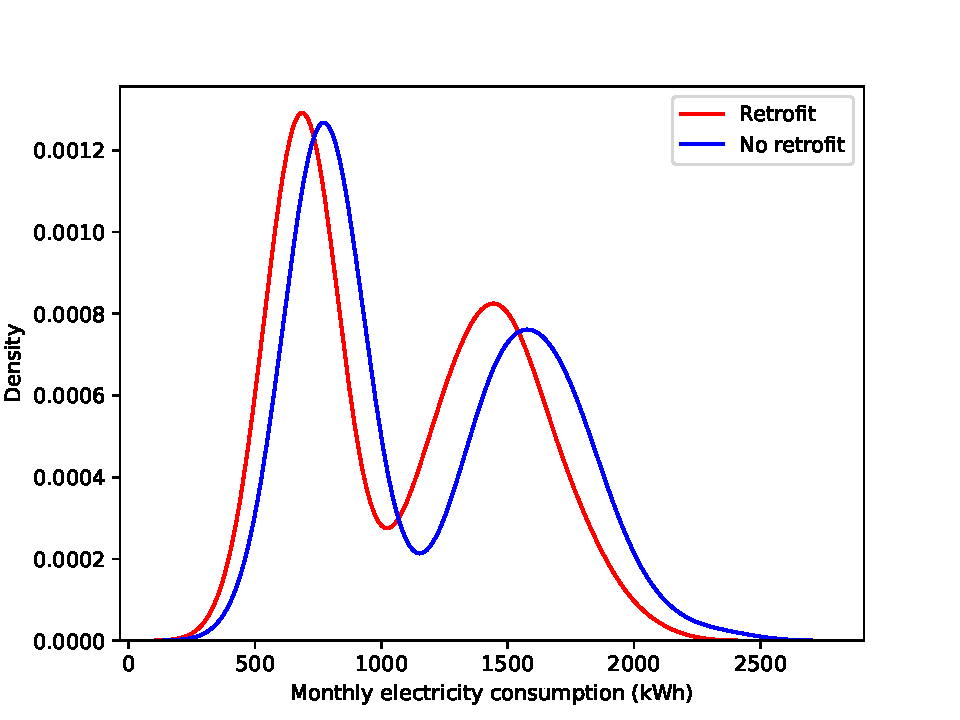
\includegraphics[scale = 0.6]{./figure/2_hist.pdf}
    \caption{Density plot of electricity consumption}
    \label{f1:hist}
\end{figure}

\subsection{OLS regression}

\begin{table}[H]\centering
\begin{threeparttable}
    \caption{OLS estimates for different computation methods}
    \label{t3:ols}
    \begin{tabular}{lccc}
\toprule
 & By Hand & Stats Model & Least Squares \\
\midrule
=1 if house received retrofit & -109.666 & -109.666 & -109.666 \\
  & (7.948) & (7.948) & (7.948) \\
Square feet of home & 0.615 & 0.615 & 0.615 \\
  & (0.006) & (0.006) & (0.006) \\
Outdoor average temperature (\textdegree F) & 3.255 & 3.255 & 3.255 \\
  & (1.924) & (1.924) & (1.924) \\
Constant & -83.603 & -83.603 & -83.593 \\
  & (154.360) & (154.360) & (154.360) \\
M.S.E. & 125.652 & 125.652 & 125.652 \\
\bottomrule
\end{tabular}

    \begin{tablenotes}
    \small \item abcd
    \end{tablenotes}
\end{threeparttable}
\end{table}

\begin{table}[H]\centering
    \begin{threeparttable}
        \caption{OLS estimates with robust S.E. for different computation methods}
        \label{t4:ols_robust}
        \begin{tabular}{lccc}
\toprule
 & By Hand & Stats Model & Least Squares \\
\midrule
=1 if retrofit & -109.666 & -109.666 & -109.666 \\
  & (7.943) & (7.943) & (7.943) \\
Square feet of home & 0.615 & 0.615 & 0.615 \\
  & (0.007) & (0.007) & (0.007) \\
Outdoor average temperature & 3.255 & 3.255 & 3.255 \\
  & (1.932) & (1.932) & (1.932) \\
Constant & -83.603 & -83.603 & -83.593 \\
  & (154.695) & (154.695) & (154.695) \\
MSE & 125.652 & 125.652 & 125.652 \\
\bottomrule
\end{tabular}

        \begin{tablenotes}
        \small \item abcd
        \end{tablenotes}
    \end{threeparttable}
    \end{table}

\section{Stata}

\subsection{Balance table}

\begin{table}[H]\centering
\begin{threeparttable}
    \caption{Balance table from Stata}
    \label{t4:balance}
    {
\def\sym#1{\ifmmode^{#1}\else\(^{#1}\)\fi}
\begin{tabular}{l*{3}{c}}
\hline\hline
                    &\multicolumn{1}{c}{Control}&\multicolumn{1}{c}{Treatment}&\multicolumn{1}{c}{P-value}\\
\hline
Electricity         &    1181.33 &    1086.75 &       0.001\\
                    &   (454.31) &   (423.96) &     [3.404]\\
Square feet of home &    1633.05 &    1657.55 &       0.572\\
                    &   (682.90) &   (686.27) &    [-0.566]\\
Outdoor average temperature&      79.89 &      79.89 &       0.987\\
                    &     (2.16) &     (1.97) &    [-0.016]\\
\hline
Observations        &         501&         499&       1,000\\
\hline\hline
\end{tabular}
}

    \begin{tablenotes}
    \small \item abcd
    \end{tablenotes}
\end{threeparttable}
\end{table}

\subsection{Scatterplot}

\begin{figure}[H]
    \centering
    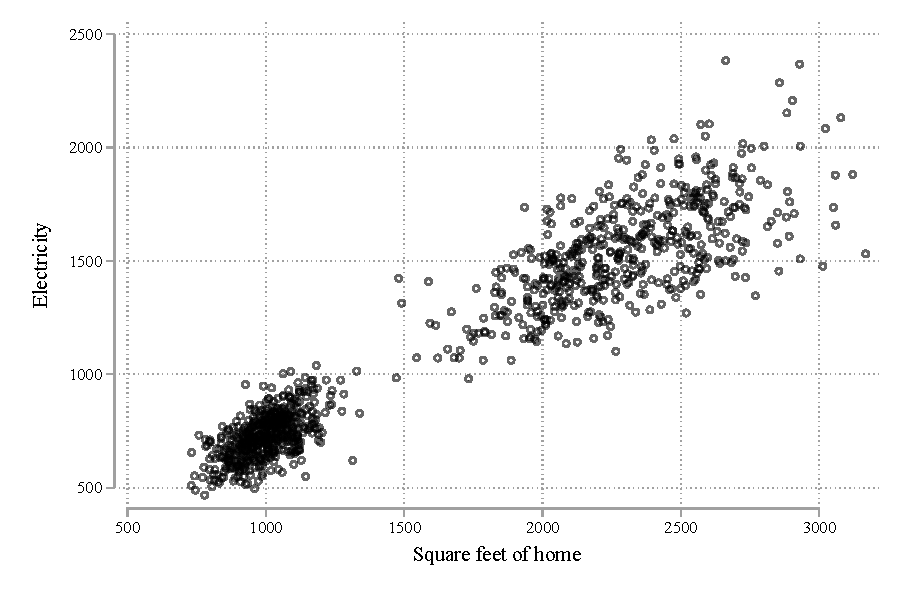
\includegraphics[scale = 1]{./figure/twoway.pdf}
    \caption{Scatterplot of electricity consumption and square feet of home}
    \label{f2:twoway}
\end{figure}

\subsection{OLS regression}

\begin{table}[H]\centering
\begin{threeparttable}
    \caption{Estimates from Stata}
    \label{t5:ols_satat}
    \begin{tabular}{l*{2}{c}}
\hline\hline
                    &\multicolumn{1}{c}{OLS}&\multicolumn{1}{c}{OLS with robust s.e.}\\
\hline
=1 if house received retrofit&    -109.666&    -109.666\\
                    &     (7.948)&     (7.943)\\
Square feet of home &       0.615&       0.615\\
                    &     (0.006)&     (0.007)\\
Outdoor average temperature (\textdegree F)&       3.255&       3.255\\
                    &     (1.924)&     (1.932)\\
Constant            &     -83.603&     -83.603\\
                    &   (154.360)&   (154.695)\\
\hline
MSE                 &     125.652&     125.652\\
\hline\hline
\end{tabular}

    \begin{tablenotes}
    \small \item abcd
    \end{tablenotes}
\end{threeparttable}
\end{table}

\cite{zm2009}

\bibliography{\bib}

\end{document}